\documentclass{webofc}
% option "twocolumn" for typesetting an article in two columns format (default one column)
% \documentclass[twocolumn]{webofc}
% 
\usepackage[varg]{txfonts}   % Web of Conferences font
\usepackage{hyperref}
\usepackage{url}
\usepackage{siunitx}
\usepackage{upgreek}
%
\usepackage{pdfpages}
\immediate\write18{pdflatex -output-directory=FirstPage FirstPage/cr_template.tex}
\usepackage{standalone}
%
% \usepackage{lineno} % for line numbers
% \linenumbers % for line numbers
%%%%%%%%%%%%%%%%%%%%%%%%%%%%%%%%%%%%%%%%%%%%%%%%%%%%%%%%%%%%%%%%%%%%%%%%%%%%%
\hypersetup{colorlinks=true,citecolor=blue,urlcolor=blue,linkcolor=blue}
%%%%%%%%%%%%%%%%%%%%%%%%%%%%%%%%%%%%%%%%%%%%%%%%%%%%%%%%%%%%%%%%%%%%%%%%%%%%%
%
% Put here some packages required or/and some personnal commands
%
\newcommand{\sm}{\ensuremath{\sim}}
%
\begin{document}
%
\includepdf[pages=1]{FirstPage/cr_template.pdf}
%
\title{Next-Generation Triggers for CMS at the HL-LHC: Toward Offline-Quality Real-Time Reconstruction}
%
% subtitle is optional
%
%%%\subtitle{Do you have a subtitle?\\ If so, write it here}
% 
\author{
  \firstname{Bruno} \lastname{Alves}\inst{1}\fnsep\thanks{\email{bruno.alves@cern.ch}}, on behalf of the CMS collaboration\footnote{Copyright 2026 CERN for the benefit of the CMS Collaboration. Reproduction of this article or parts of it is allowed as specified in the CC-BY-4.0 license.}
}
% 
\institute{
    CERN, 1211 Geneva 23, Switzerland
}
%
\abstract{The Next-Generation Trigger (NGT) program for the CMS High-Level Trigger (HLT) aims at enabling full-rate recording of all the events accepted by the Level-1 Trigger at \SI{750}{\kilo\hertz} via a dedicated NGT Scouting stream, performing complete physics event reconstruction with no additional filtering.
  Reconstructed objects are stored directly in a lightweight NanoAOD format, delivering analysis-ready data at unprecedented throughput, while minimizing the per-event footprint.
  To guarantee offline-quality physics performance without storing raw detector information, major advances in HLT reconstruction have been introduced.
  The Patatrack pixel-tracking upgrade -- extended to the first pixel-strip barrel layers of the Outer Tracker -- yields a competitive efficiency across the full detector, while showcasing a sharply reduced fake rate of up to $\sim$25\% in the barrel region.
  It also exhibits timing gains of $\sim$34\%, by eliminating a full Kalman-Filter-based tracking iteration.
  In addition, improvements in the HLT muon reconstruction chain, based on single L1-seeded Inside-Out tracking with targeted recovery, also achieve a competitive efficiency, while reducing the fake rate by up to $\sim$35\%.
  Together, these developments pave the way to the real-time production of offline-quality physics objects at extreme trigger rates, opening new discovery potential for signatures that are currently limited by bandwidth.
}
%
\maketitle
%
\section{The NGT Scouting Stream at the HL-LHC}
\label{intro}
The two-tiered online selection of LHC data by the Level-1 Trigger (L1T) and the High-Level Trigger (HLT) at the Compact Muon Solenoid (CMS) experiment \cite{cms} is essential to reduce the \SI{40}{\mega\hertz} LHC bunch-crossing rate to a bandwidth and storage footprint that is sustainable for offline processing and analysis.
The L1T acts as the first filtering stage and has access to only a limited, coarse-grained detector readout; in Phase~2, it will operate with a fixed latency of \SI{12.5}{\micro\second} per event.
This is followed by the HLT, which only runs on the events accepted by the L1T, and has access to the full detector readout, operating with an average processing-time budget of the order of \SI{1}{\second} per event in Phase~2.
Despite the overwhelming reduction of data rate between these two stages, the trigger system provides an efficient online selection of rare physics processes. \par
%
Innovative trigger strategies have been employed in CMS since its inception, and quite intensely during Run~3~\cite{scout}.
One such strategy, \textit{data parking}, addresses the limited availability of prompt computing resources by storing the raw data while deferring the full reconstruction until resources are again available.
Another strategy, \textit{data scouting}, which this work discusses, addresses both storage and computing limitations by reconstructing events collected by related scouting streams only up to HLT level.
The resulting scouting output is a reduced analysis-ready data format which bypasses the offline reconstruction.
These strategies enable a significant reduction of trigger thresholds with respect to the standard data stream, and thus the exploration of phase-space regions otherwise inaccessible, at the cost of a degradation in the resolution of physics objects. \par
%
The High-Luminosity LHC (HL-LHC) is scheduled to start taking data in 2030, reaching unprecedented instantaneous luminosities of \sm\SI{7.5e34}{\per\square\centi\meter\per\second}, corresponding to a \sm3.5 times increase over peak Run~3 conditions, and an average pileup of 200, compared to \sm60 in Run~3.
Many CMS subdetectors will undergo significant upgrades, ranging from electronics-only updates, as for the barrel electromagnetic calorimeter, to complete overhauls, as will be the case for the endcap calorimeter.
The trigger system will therefore have to operate in an extremely challenging environment, driven by the overall increase in detector data volume and event complexity.
Data scouting and parking techniques will be extensively explored and expanded during the HL-LHC era \cite{scout}. \par
%
The Next-Generation Trigger (NGT) project~\cite{ngt} aims to extend the physics reach of CMS beyond what is achievable with the baseline Phase~2 trigger system, by making lightweight, offline-like reconstructed objects available in real time.
One of its main goals is to pursue a next-generation scouting strategy targeting the largest ever recorded scouting bandwidth, while improving on the intrinsically lower per-object precision associated with scouting-quality reconstruction.
This builds on the demonstrated success of scouting techniques since their introduction in CMS, and their considerable expansion during Run~3 \cite{scout}.
Concretely, the goal within NGT is to reconstruct \emph{all} events accepted by the L1T, at \SI{750}{\kilo\hertz}, and record them in a compact, analysis-ready \texttt{NanoAOD}-like data format, via a dedicated NGT Scouting stream (see Fig.~\ref{fig:concept}).
The baseline scouting strategy, instead, is currently aiming for a \SI{225}{\kilo\hertz} rate~\cite{octdr}, corresponding to \SI{\sim 70}{\percent} less than the NGT proposal.
As an additional comparison, the standard HLT approach (also in Fig.~\ref{fig:concept}), which consists of selecting high-interest events and writing out the full raw detector data for later offline analysis, is planned to work at \SI{\sim 15}{\kilo\hertz}.
Attaining a scouting stream at \SI{750}{\kilo\hertz} requires both the development of new reconstruction algorithms and the redesign of existing ones, so that the resulting throughput remains within constraints, in terms of compute, storage, and, ultimately, cost.
As part of this effort, the target fractions of the HLT code to be offloaded to GPUs are 50\% (80\%) by the start of Run~4 (Run~5)~\cite{hlttdr}. \par
%
\begin{figure}[h]
\centering
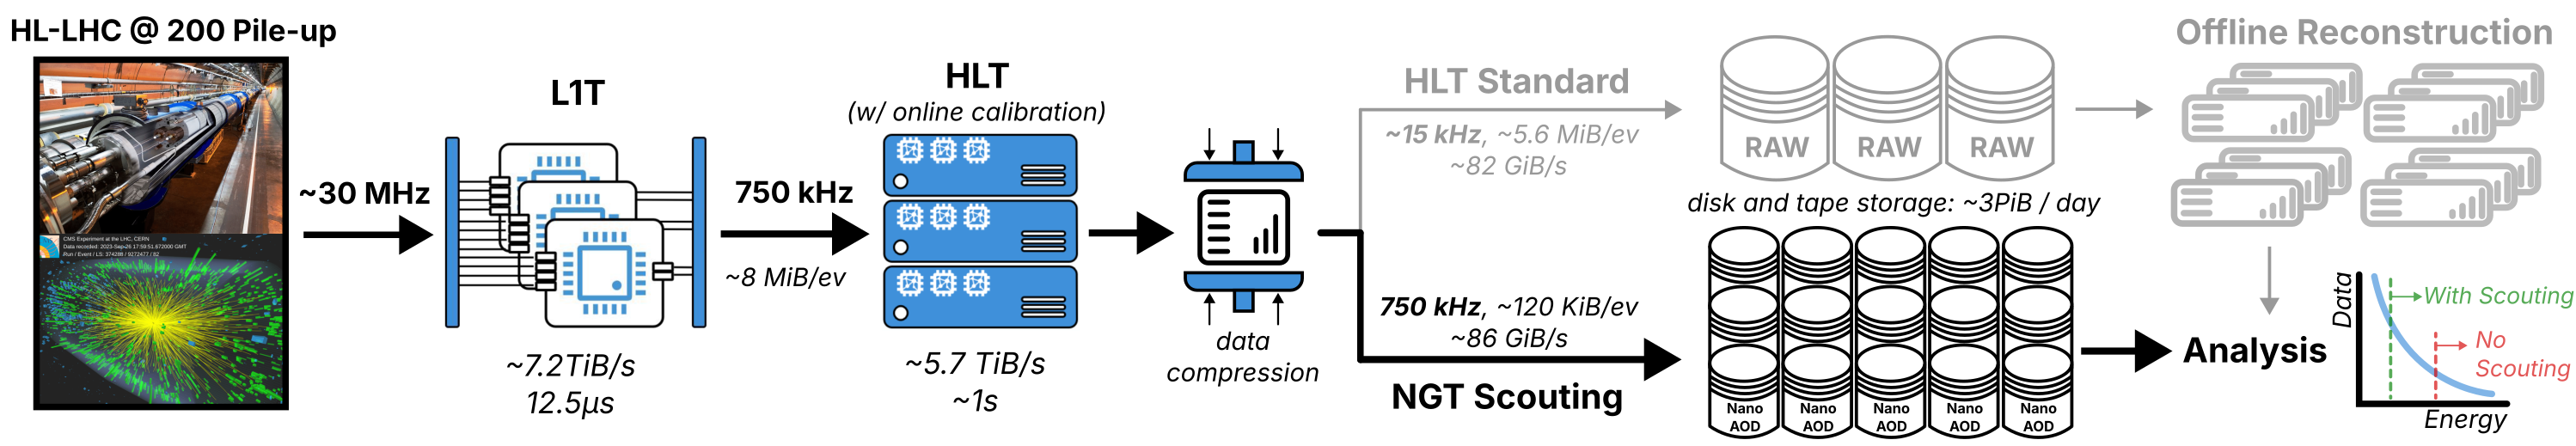
\includegraphics[width=1.\textwidth]{ngtconcept}
\caption{Simplified schematic overview of the trigger processing chain in CMS during Phase~2, from the collision rate at the HL-LHC with 200 PU to the final analysis step.
  Both the HLT Standard and the NGT Scouting paths are shown, with current expected rates and throughput values.
  The HLT Standard approach selects high-interest events at \SI{\sim 15}{\kilo\hertz} and writes out the full detector raw data for later offline analysis.
  The NGT Scouting path reconstructs all events accepted by the L1T at \SI{750}{\kilo\hertz}, with no additional filtering, and stores the events directly in a compact, analysis-ready \texttt{NanoAOD}-like data format.}
\label{fig:concept}
\end{figure}
%
NGT also plans to innovate on how calibrations are performed at the HLT.
In CMS, different calibration constants need to be updated at different frequencies, ranging from minutes to weeks.
While offline calibration workflows are typically allowed to take up to 48 hours, their online counterparts must be derived much faster, introducing additional algorithmic and operational challenges.
NGT is currently developing a real-time calibration strategy for the HLT that targets a resolution comparable to what is achieved offline.
This idea builds on a demonstrator system which buffers $\sim$1\% of the data stream and applies improved calibrations before the HLT reconstruction, successfully operated during Run~3 \cite{demonstrator}. \par
%
The remainder of this work focuses on two of the key algorithmic developments that will help the NGT Scouting stream to approach an offline-quality reconstruction: the extension to the Outer Tracker and GPU-based acceleration of the pixel-based tracking reconstruction algorithm (Sec.~\ref{sec:track}), and the redesign of the HLT muon reconstruction chain (Sec.~\ref{sec:muon}).
%
\section{The Extended Patatrack Pixel Tracking Algorithm}
\label{sec:track}
%
The CMS Phase~2 tracker (see Fig.~\ref{fig:detector}) will include \sm2.2 billion readout channels, a \sm16-fold increase compared to Run~3~\cite{trackerphase2}.
This dramatic rise in detector complexity makes tracking the single largest contributor to the HLT reconstruction time, accounting for more than 40\% of the total processing budget, and therefore the primary target for new algorithmic and heterogeneous developments.
The readout channels are divided between the Inner Tracker (IT), comprising high-density silicon pixel modules arranged across 4 barrel layers and 12 disks per endcap, and the Outer Tracker (OT), which features macro-pixel-plus-strip (PS) and double-strip (2S) modules across 6 barrel layers and 5 disks per endcap.
In the barrel, the first three layers of the OT hold PS modules, while the remaining 3 exterior layers contain 2S modules. \par
%
\begin{figure}[h]
\centering
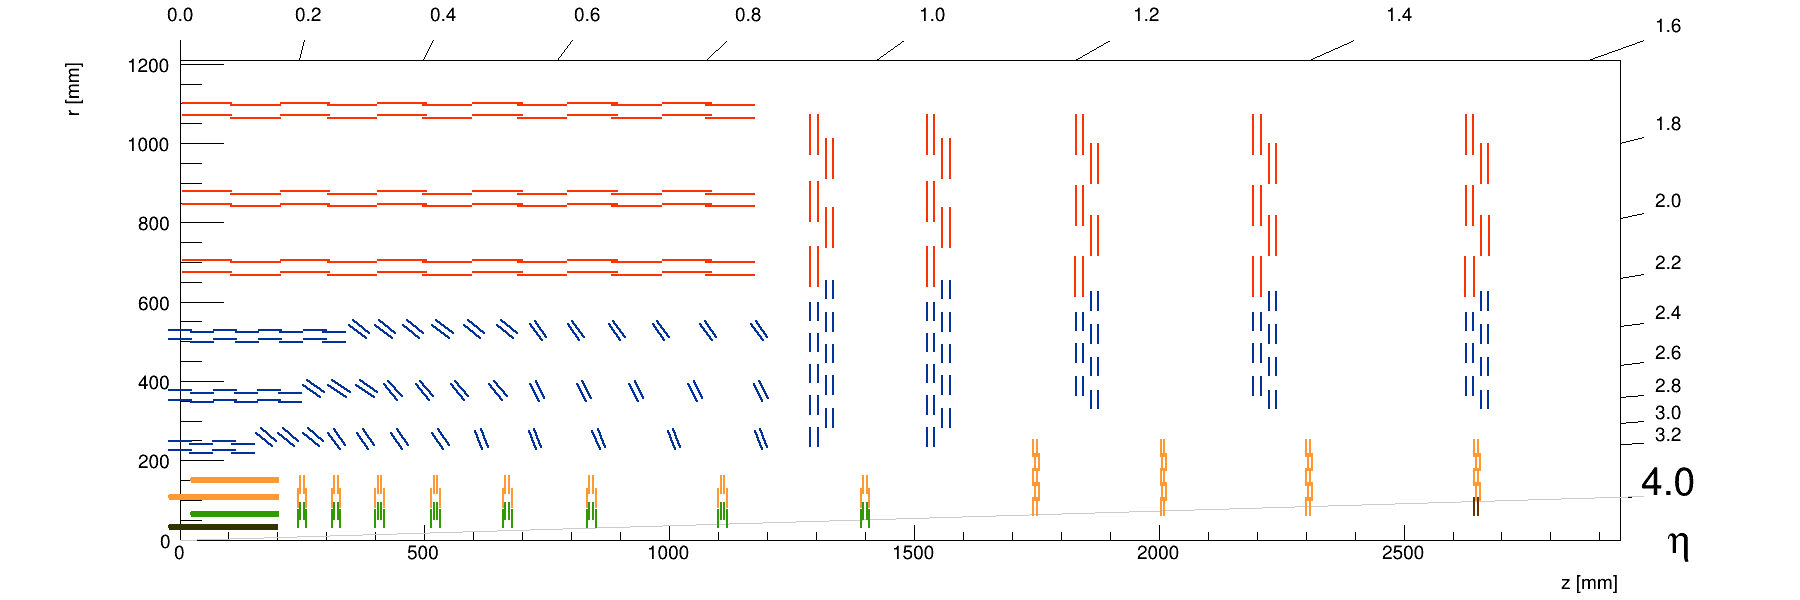
\includegraphics[width=1.\textwidth]{Phase2_Tracker_1Quarter}
\caption{Schematic view of a quarter of the Phase-2 CMS Tracking Detector in an $r$ versus $z$ projection.
  Each line segment represents the centre of a module, with pairs of parallel lines showing separate modules staggered along the azimuthal angle.
  The Inner Tracker is composed of a total of 4000 sensors of three types with $25\times100$ \unit{\micro\meter\squared} pitch: 3D pixels with 1 chip per sensor (black), planar pixels with 2 chips per sensor (green) and planar pixels with 4 chips per sensor (orange).
  The Outer Tracker is composed of a total of 13200 double-sensor modules of two types: 2S modules (red) made of 2 microstrip sensors with \SI{90}{\micro\meter} pitch and PS modules (blue) made of one macro-pixel sensor with $1.5\times0.1$ \unit{\milli\meter\squared} pitch and one micro-strip sensor with \SI{100}{\micro\meter} pitch. 
}
\label{fig:detector}
\end{figure}
%
Tracking algorithms should prioritize a high efficiency, low fake rate and fast execution time.
The reconstruction of full tracks proceeds through three sequential steps:
%
\begin{itemize}
\item \textit{Seeding}: using the Cellular Automaton (CA) algorithm, the hits from the Inner Tracker (IT) pixel layers are combined into short pixel-only track candidates to determine the approximate location and direction of each particle.
  The heterogeneous \textit{Patatrack} pixel tracking algorithm \cite{patatrack} has been developed to provide a GPU-friendly and faster implementation of the CA.
\item \textit{Building}: the seeds are extended into full tracks using OT hits via the Combinatorial Kalman Filter (CKF) algorithm \cite{ckf}.
\item \textit{Fitting}: track parameters are extracted via a fit, also performed by CKF.
\end{itemize}
%
\noindent Optionally, fitted tracks can be selected using quality-based criteria, such as neural network scores. \par
%
In this work we implement and study the following three tracking configurations:
%
\begin{itemize}
\item \texttt{Legacy}: the reference tracking reconstruction sequence, running two sequential CA-seeded iterations (IT-only quadruplets, followed by triplets), with track building and fitting performed entirely by CKF.
  This tracking reconstruction configuration runs sequentially and is CPU-only.
\item \texttt{Patatrack}: functionally equivalent to \texttt{Legacy}, with the same two IT-only quadruplet and triplet iterations, but the pixel-seed creation step is offloaded to the GPU-compatible \textit{Patatrack} algorithm, while the building and fitting steps remain unchanged.
\item \texttt{Extended Patatrack}: a fast, scouting-oriented configuration in which a single \textit{Patatrack} seeding iteration is run using \emph{both} IT and macro-pixel hits from PS modules, requiring at least four hits in total, of which at least two must belong to the IT.
  Only the barrel section of the pixel OT is considered.
  The three outermost strip layers of the OT are also not considered.
  The resulting extended, GPU-compatible pixel tracks are used directly as final tracks.
  CKF is not run, and no separate full-track building or second iteration is performed.
\end{itemize}
%
\subsection{Performance measurements}
\label{sec:trackperf}
\begin{figure}[h]
\centering
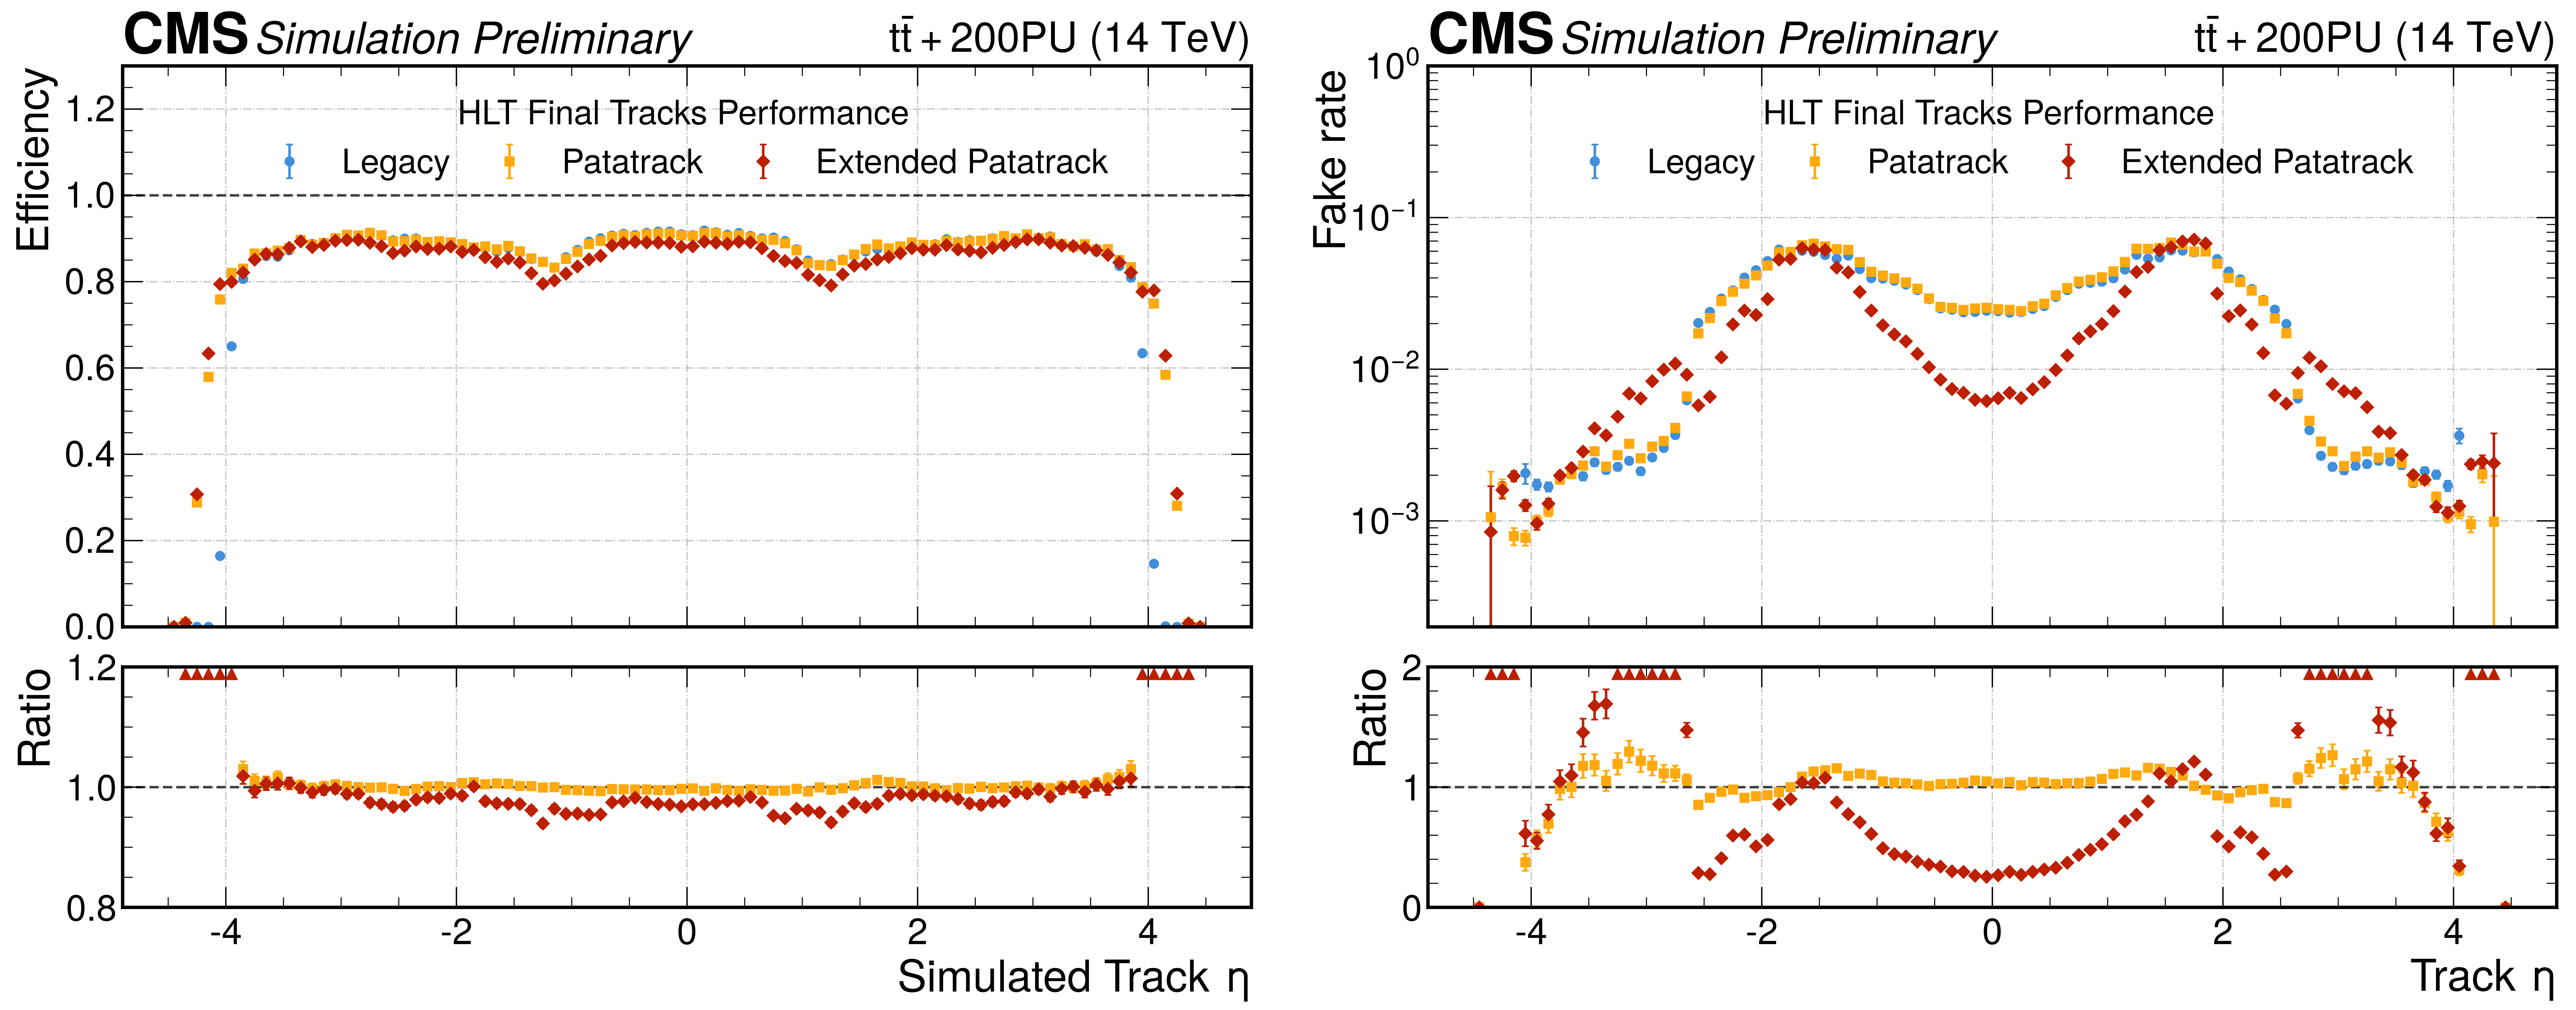
\includegraphics[width=1.\textwidth]{track_perf}
\caption{Full tracking efficiency performance as a function of the pseudorapidity ($\eta$) of the simulated track.
  The left (right) figure shows the tracking efficiency (fake rate) of the \texttt{Legacy} (blue), \texttt{Patatrack} (orange), and \texttt{Extended Patatrack} (red) configurations.
  The \texttt{Extended Patatrack} configuration achieves a very strong reduction of the fake rate in the barrel region compared to the two other configurations, at the cost of a relatively modest 5\% relative efficiency reduction, despite exploiting substantially less detector information. Taken from Ref.~\cite{ngtdps}.
}
\label{fig:trackperf}
\end{figure}
%
The three configurations presented in Section~\ref{sec:track} are compared in terms of physics and timing performance in Fig.~\ref{fig:trackperf}.
There, the tracking efficiency is defined as the fraction of simulated tracks matched to at least one reconstructed track, where a reconstructed track is considered matched to a simulated track if more than 75\% of the associated hits originate from the simulated track.
The fake rate is defined as the fraction of reconstructed tracks not matched to any simulated track.
We observe that the \texttt{Extended Patatrack} configuration significantly reduces the fake rate in the barrel region ($|\eta| < 1.47$) by up to $\sim$25\% compared to the other two configurations.
Simultaneously, its efficiency in the endcaps remains compatible with the baseline within 5\%, while in the barrel, especially near the transition regions ($|\eta| \approx 1.5$), both \textit{Patatrack}-based configurations achieve up to $\sim$10\% higher efficiency.
Moreover, for very high $|\eta|$ values, the two \textit{Patatrack} configurations achieve a higher efficiency.
It should be noted that these measurements do not consider the strip section of the OT, nor the pixel-strip modules in the endcaps.
The results shown in Fig.~\ref{fig:trackperf} illustrate the potential of pixel-based tracking to complement full offline-quality tracking at the HLT. \par
%
To assess the computational feasibility of the NGT Scouting strategy, the average per-event processing time spent in the different HLT modules was measured for each of the three tracking configurations, and is shown in Fig.~\ref{fig:timing}.
The timing was evaluated on a sample of 900 $t\bar{t}$ events, stored in a single file and simulated at an average pileup of 200, of which 89.5\% pass at least one L1 seed and are therefore processed by the HLT.
Each measurement was preceded by four (discarded) I/O-only warm-up runs and was repeated three times, using 16 parallel jobs, each independently processing the full event sample; input files were pre-loaded into the operating system cache beforehand to emulate real data-taking conditions.
The measurement was carried out on a dedicated machine equipped with two AMD EPYC 9534 CPUs, providing a total of 256 logical cores ($2~\text{sockets} \times 64~\text{physical cores} \times 2~\text{threads}$).
The node is also equipped with 4 NVIDIA L40 GPUs, which are disabled for CPU-only setups and enabled for CPU+GPU setups.
With GPUs enabled, the jobs are distributed in a round-robin fashion, leading to 4 jobs per GPU.
The CPU-only \texttt{Legacy} result is identical in both plots since this configuration includes no heterogeneous implementation.
The results show that the \texttt{Extended Patatrack} configuration yields an 18\% speed-up relative to the \texttt{Patatrack} configuration in the average processing time per event for the CPU-only setup (left), already including the additional cost of incorporating OT macro-pixel hits.
The speed-up is due to the use of pixel-only tracks and the removal of both the second iteration and the CKF steps.
The same reasons lead to a 34\% speed-up of the \texttt{Extended Patatrack} configuration relative to the \texttt{Patatrack} configuration when GPUs are enabled (right), on top of the 8\% throughput speed-up already provided by the \textit{Patatrack} algorithm on GPU relative to the CPU setup.
The GPU-based pixel-tracking step thus becomes negligible in terms of processing time, as shown by the green entries for ``Pixel Triplets'', ``Pixel Quadruplets'' and ``Tracking'' modules. \par
%
\begin{figure}[h]
\centering
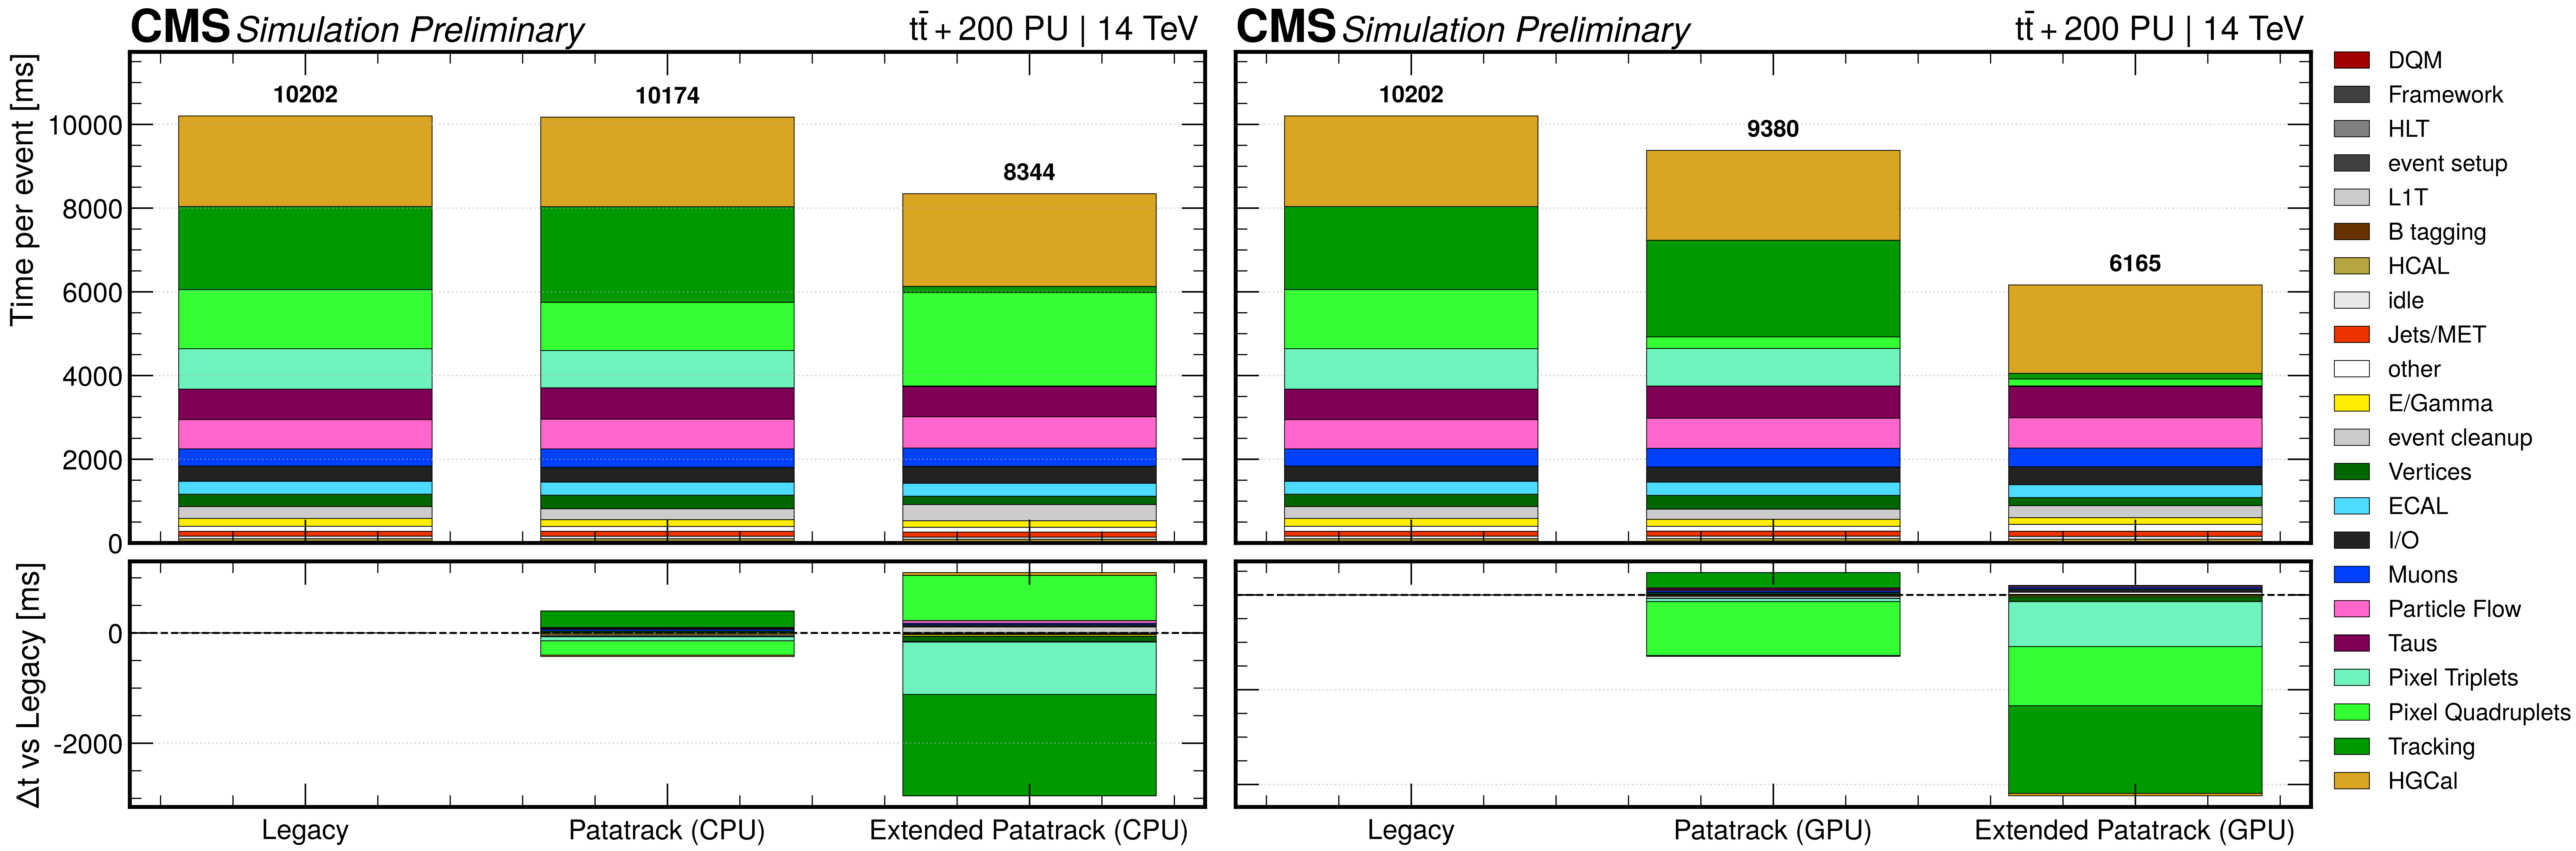
\includegraphics[width=1.\textwidth]{timing}
\caption{Average processing time spent per event in the different HLT reconstruction components of the NGT Scouting stream, for the \texttt{Legacy}, \texttt{Patatrack}, and \texttt{Extended Patatrack} configurations, running on CPU only (left) or with GPU offloading enabled (right).
  The CPU-only \texttt{Legacy} result is identical in both plots, since this configuration includes no heterogeneous implementation.
  The \texttt{Extended Patatrack} configuration yields an 18\% speed-up relative to the \texttt{Patatrack} configuration in the average processing time per event for the CPU-only setup -- already including the additional cost of incorporating OT macro-pixel hits -- owing to the use of pixel-only tracks and the removal of both the second iteration and the CKF steps.
  The same configuration reaches a 34\% speed-up relative to the \texttt{Patatrack} configuration when GPUs are enabled, for identical reasons, on top of the 8\% higher throughput of the \textit{Patatrack} algorithm on GPUs, rendering the pixel-tracking step essentially negligible in terms of processing time, as shown by the green entries for ``Pixel Triplets'', ``Pixel Quadruplets'' and ``Tracking'' modules.
  Taken from Ref.~\cite{ngtdps}.
}
\label{fig:timing}
\end{figure}
%
\section{Rethink and Optimize the Muon Tracking}
\label{sec:muon}
%
The default HLT Phase~2 muon reconstruction in CMS builds objects in the tracker and in the muon chambers: standalone muons, using muon-only seeds, and tracker muon tracks, using L1T seeds with both muon and tracker information.
The reconstruction of tracker muon tracks consists of two steps: the Inside-Out (IO) step and the Outside-In (OI) step.
The IO step uses L1T seeds to define regions of interest in the IT, where two tracking iterations are run, following the logic of the \texttt{Legacy} configuration for pixel tracks (see Sec.~\ref{sec:track}).
Importantly, pixel tracks are recomputed.
The OI starts instead from OT seeding regions (built from the direction of standalone muons), where a CKF approach is used to produce a trajectory connecting hits in the direction of the IT.
Tracker muon tracks are then matched to standalone muons to produce global muons, by comparing parameters after propagating both trajectories to a common surface.
Finally, an identification procedure is applied to HLT muon candidates, producing the final HLT muons. \par
%
This work proposes and validates major updates to the HLT muon reconstruction chain.
Firstly, we show that removing muon seeds does not impact physics performance.
A single set of L1T seeds is now considered, requiring no further match with other seed collections, and is directly used to produce standalone muons, simplifying the reconstruction.
Secondly, the IO step is overhauled: within tracker seed regions, \texttt{Legacy} pixel tracks are replaced by pixel tracks created with the \texttt{Extended Patatrack} configuration plus a CKF propagation step to the OT.
This equates to moving from two iterations to a single iteration IO step.
Furthermore, instead of being recomputed, extended pixel tracks selected within a given seed region are recycled from the ones already computed for tracking purposes.
Finally, the IO and OI steps are chained such that the OI sequence acts solely as a recovery mechanism for muon candidates missed during the IO step, thereby avoiding duplicate reconstruction. \par
%
The performance improvements brought by the updates to the muon tracking were measured in simulated $\text{Z}\rightarrow\upmu\upmu$ events under HL-LHC conditions, with an average pileup of 200.
The efficiency is here defined as the fraction of simulated target muons that are matched to a reconstructed muon object, where a matching is considered if the two objects share more than 75\% of their hits.
The fake rate is defined as the ratio of reconstructed muons not matched to any simulated target muon over the total number of reconstructed muons.
The muons are reconstructed by merging the IO and OI muon track collections, that is, also taking into account the OI recovery step.
Only simulated muons produced in the Z decay within the detector acceptance conditions are considered.
In particular, simulated muons must satisfy $|\eta| \leq 2.4$ and $p_\text{T} > \SI{0.9}{\giga\eV}$.
Performance results are shown in Fig.~\ref{fig:muonperf} in terms of reconstruction efficiency (left) and fake rate (right), where the new single iteration IO step is compared to the legacy, two-iteration IO approach.
We can observe that the new iteration, in orange, achieves an efficiency of $\sim$95\%, comparable to the default blue one.
At the same time, the fake rate is reduced by $\sim$20\% in the central part of the barrel section, reaching a $\sim$35\% improvement at $|\eta| \sim 1.2$.
Smaller improvements of $\sim$5\% or less can also be observed in the endcaps.
The results show that the current updated approach holds significant potential to be considered for the muon reconstruction at HLT.
Parameter optimization is ongoing to further boost performance. \par
%
\begin{figure}[h]
\centering
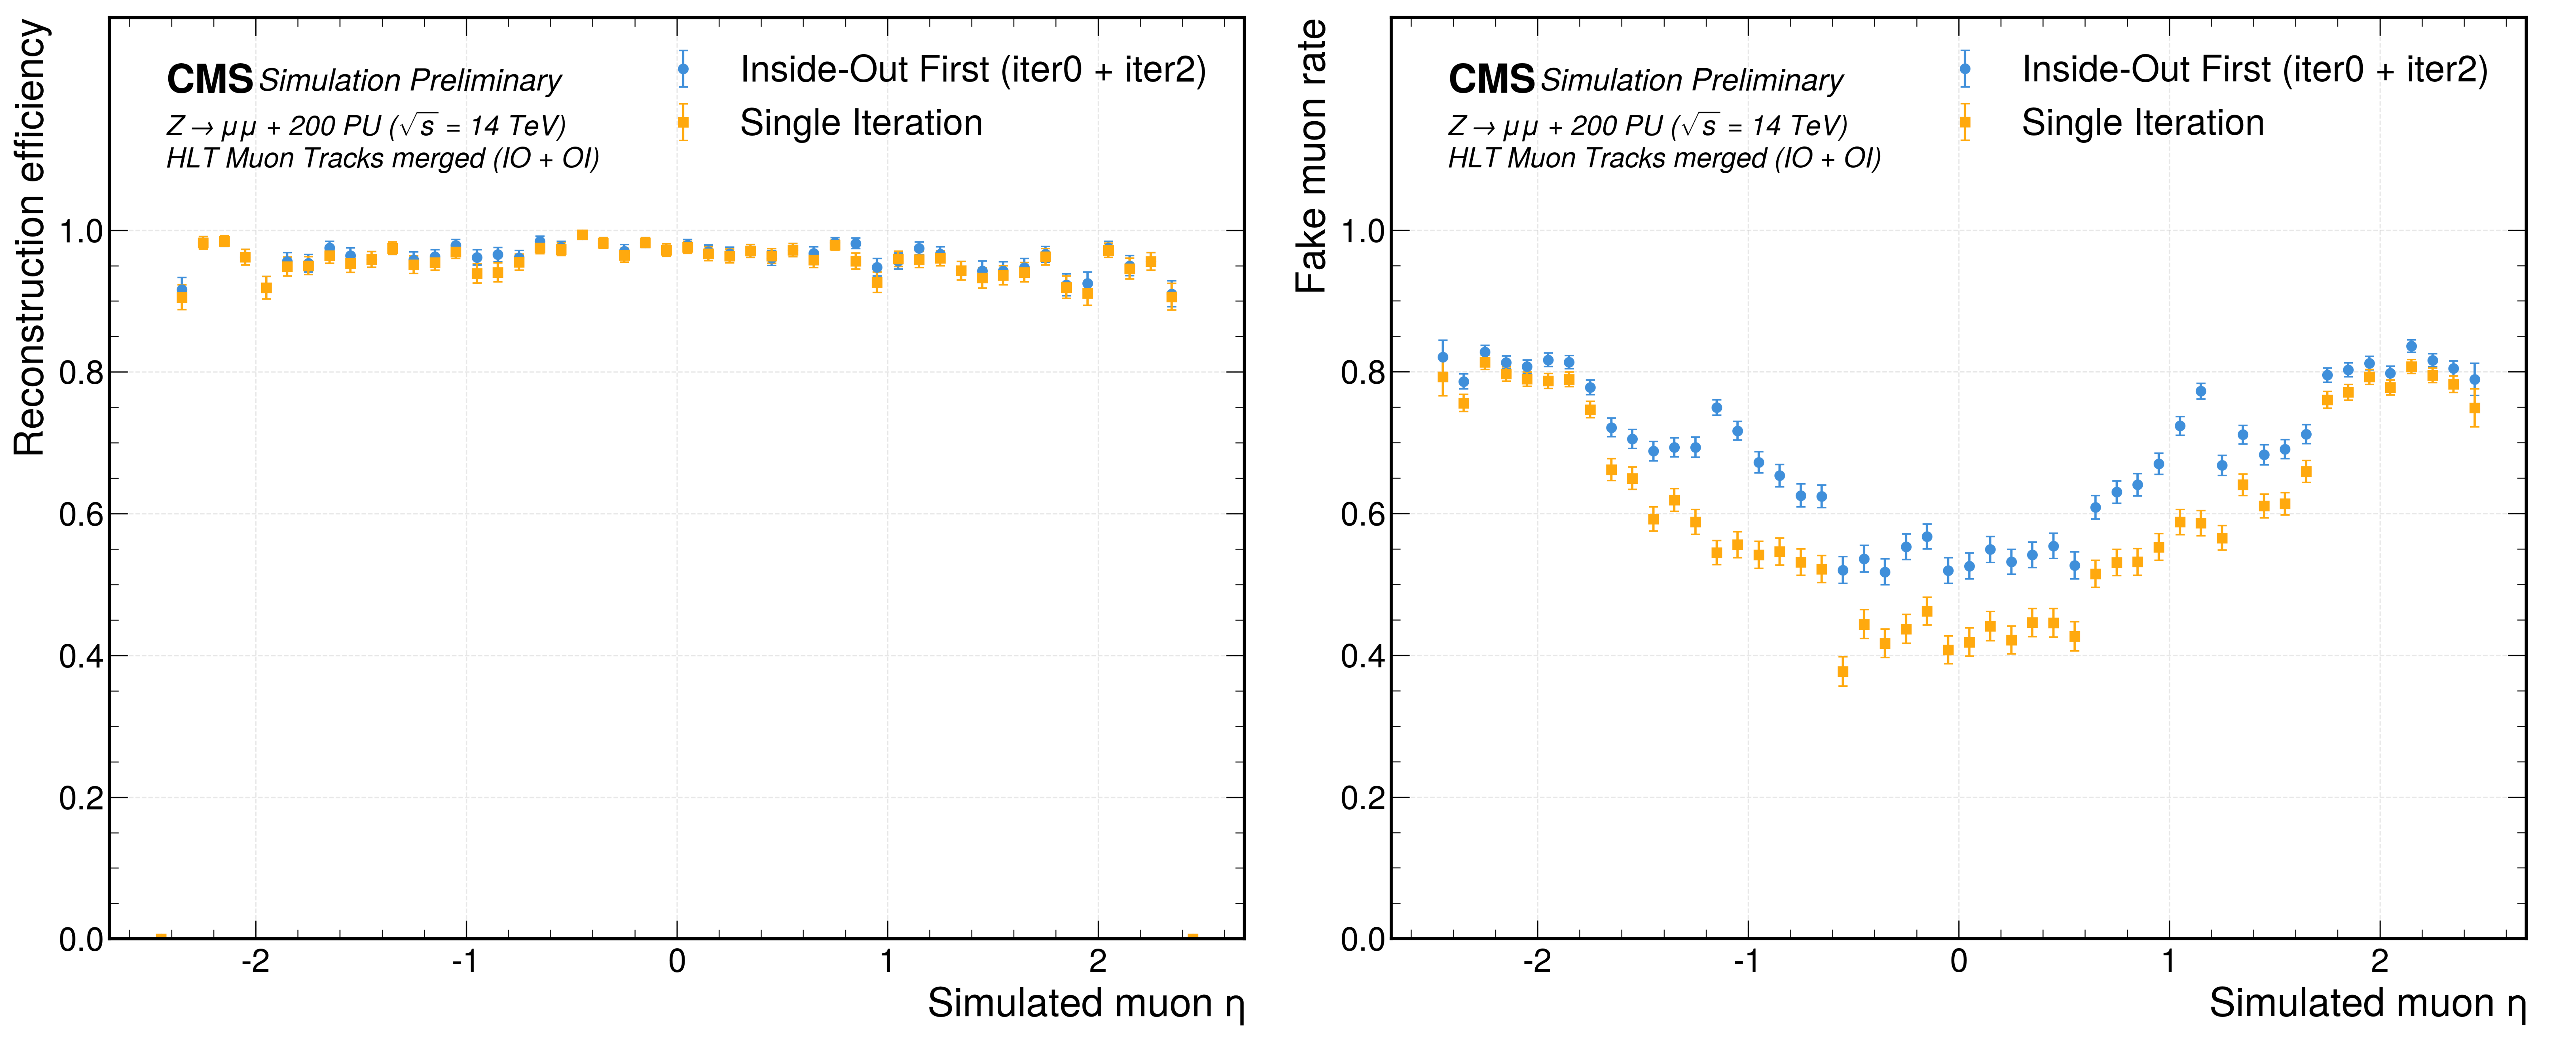
\includegraphics[width=1.\textwidth]{muon_perf}
\caption{Physics performance of the new single iteration IO step, measured in simulated $\text{Z}\rightarrow\upmu\upmu$ events under HL-LHC conditions, with an average pileup of 200.
  Simulated muons must originate from the Z decay and must satisfy $|\eta| \leq 2.4$ and $p_\text{T} > \SI{0.9}{\giga\eV}$.
  The two distributions represent the HLT muon reconstruction by running first the IO step, and then the OI as a recovery step.
  The blue distribution uses the \texttt{Legacy} configuration for the IO step, while the orange distribution considers the single iteration approach using the \texttt{Extended Patatrack} configuration for the IO step.
  The left (right) plot shows the reconstruction efficiency (fake rate) of HLT Muon tracks as a function of the simulated muon pseudorapidity $\eta$.
  The efficiency curves are comparable.
  The fake rate is reduced by $\sim$20\% in the central part of the barrel section, reaching a $\sim$35\% improvement at $|\eta| \sim 1.2$.
  Smaller improvements of $\sim$5\% or less can also be observed in the endcaps.
  Taken from Ref.~\cite{muonphase2}.
}
\label{fig:muonperf}
\end{figure}
%
\section{Conclusions}
\label{sec:conclusions}
%
This work presents the ambitious NGT scouting strategy for the HLT system of CMS during the HL-LHC phase, introducing its challenges and some of the techniques used to make it possible.
In particular, we discuss substantial improvements of the online reconstruction chain of tracks and muons, in terms of physics and computing performance.
Tracking has historically been the largest contributor to execution time in the CMS HLT reconstruction, due to the extremely high channel count, which will be further increased for the HL-LHC.
While achieving a clear reduction in processing time, the presented pixel tracking results remain competitive with full tracking.
The same positive behaviour is also present in the HLT muon reconstruction, where several improvements are leading to faster algorithms without strongly impacting physics performance.
Current and future studies are being undertaken to further enhance existing algorithms, which should lead to a speed and efficiency increase in the next few years. \par
%
The ultimate goal for HL-LHC reconstruction in CMS is to achieve performance that matches or exceeds current capabilities, while simultaneously attaining the execution speed needed to turn the NGT scouting strategy into reality.
In the case of pixel tracking, this requires at least matching the performance currently delivered by full track reconstruction.
Should NGT scouting at \SI{750}{\kilo\hertz} prove to be too ambitious, the proposed improvements can still be integrated into the standard High-Level Trigger (HLT) reconstruction sequence or adapted for the more conservative HLT scouting approach planned at \SI{225}{\kilo\hertz} \cite{octdr}.
Given existing similarities, the NGT improvements are also expected to benefit the offline reconstruction chain. \par
%
% BibTeX or Biber users please use (the style is already called in the class, ensure that the "woc.bst" style is in your local directory)
% \bibliography{your_bib_file} % Replace "your_bib_file" with the actual name of your .bib file
% Non-BibTeX users please use
\begin{thebibliography}{}
% and use \bibitem to create references.
%
% Journal Author, Article title. Journal \textbf{Volume}, page numbers (year). \url{https://doi.org/Article-DOI-number}
\bibitem{cms}
  The CMS Collaboration. ``The CMS Experiment at the CERN LHC''. In: JINST 3 (2008), S08004. DOI: \url{https://doi.org/10.1088/1748-0221/3/08/S08004}.
\bibitem{scout}
  The CMS Collaboration, ``Enriching the physics program of the CMS experiment via data scouting and data parking''. Physics Reports Volume 1115, 17 April 2025, Pages 678-772. \url{https://doi.org/10.1016/j.physrep.2024.09.006}
\bibitem{ngt}
  Next Generation Triggers. ``NGT Evaluation Report - 2025. CERN''. DOI: \url{https://doi.org/10.17181/dvqah-g0f70}
\bibitem{octdr}
  The CMS Collaboration, ``CMS Offline Software and Computing for HL-LHC, Conceptual Design Report''. \url{https://cds.cern.ch/record/2957472}  
\bibitem{hlttdr}
  The CMS Collaboration. ``The Phase-2 Upgrade of the CMS Data Acquisition and High Level Trigger''. \url{https://cds.cern.ch/record/2759072/}
\bibitem{demonstrator}
  The CMS Collaboration, ``Next Generation Triggers Demonstrator: Time Variation of the Calibrations and System Monitoring''. \url{https://cds.cern.ch/record/2950076}
\bibitem{trackerphase2}
  The CMS Collaboration, ``The Phase-2 Upgrade of the CMS Tracker''. \url{https://cds.cern.ch/record/2272264}
\bibitem{ckf}
  R. Mankel. ``A concurrent track evolution algorithm for pattern recognition in the HERA-B main tracking system''. Nucl. Instrum. Methods A395 (1997) 169. \url{https://doi.org/10.1016/S0168-9002(97)00705-5}
\bibitem{ngtdps}
  The CMS Collaboration, ``Computing and physics performance of a high-throughput NGT Scouting stream for the HLT Phase-2 Upgrade''. \url{https://cds.cern.ch/record/2956836}
\bibitem{muonphase2}
  The CMS Collaboration, ``Muon Tracking at the CMS High-Level Trigger for the HL-LHC Upgrade''. \url{https://cds.cern.ch/record/2950077}
\bibitem{patatrack}
  A. Bocci et al. ``Heterogeneous Reconstruction of Tracks and Primary Vertices With the CMS Pixel Tracker''. Frontiers in Big Data Volume 3 - 2020 (2020). ISSN: 2624-909X. DOI: \url{https://doi.org/10.3389/fdata.2020.601728}. url: \url{https://arxiv.org/abs/2008.13461}.
%  
% Format for books
% \bibitem{RefB}
% Book Author, \textit{Book title} (Publisher, place, year) page numbers
%
\end{thebibliography}
%
\end{document}
